\subsubsection{O que é diagrama de pacote}
É uma forma de organizar um modelo de representação de um sistema com uma hierarquia bem definida de dependência.

Pode ser organizado aglutinando-se elementos os quais provavelmente mudarão juntos à medida que o sistema for modificado ou os quais podem ser reutilizados em partes do projeto. 

\subsubsection{Estrutura do diagrama de pacote}
Cada pacote é representado por uma pasta que contém outros elementos (que precisam ser \textit{packageable}).

A relação de contenção pode ser simbolizada de duas formas diferentes: aninhando-se os elementos dentro de uma pasta ou utilizando o símbolo de retículo (também chamado de gratícula ou, em inglês, \textit{crosshair})

Todo elemento contido em um pacote é indissociável deste, por isso todo pacote define um \textit{namespace}, isto é, um ambiente onde elementos diferentes não podem ter nomes iguais, senão ocorrerá algum tipo de conflito.

\subsubsection{Importação}
No diagrama de pacote é possível fazer \textit{package import} ou \textit{element import} para compor um certo pacote.

Quando uma importação é feita, alguns cuidados devem ser tomados quanto a nomes conflitantes. Deve-se, basicamente, garantir que: 

\begin{itemize}
    \item Caso haja conflito entre um elemento-filho do pacote importador e o elemento importado, deve-se usar um pseudônimo(\textit{alias}) para desambiguar a importação
    
    \item Caso dois elementos de pacotes importados tenham nomes iguais, eles simplesmente não podem ser importados para aquele \textit{namespace}.
\end{itemize}

Elementos de um pacote podem ser públicos ou privados, e isso é definido por notas explicativas dentro do diagrama, pois o SysML ''não possui notação gráfica para visibilidade, por isso são usadas as notas anexadas aos símbolos'' \textsuperscript{[1]}

A importação em diagramas de pacote é simbolizada por uma seta que vai do importador para o importado, com a \textit{keyword} \textit{<<import>>} quando o elemento importado é público e \textit{<<access>>} quando é privado.


\subsubsection{Onde é utilizado}
Um exemplo intimamente relacionado com a Computação pode ser encontrado no \textit{standard} de uma linguagem de programação. 

A modularização que as bibliotecas básicas da linguagem Java oferece, por exemplo, pode ser representada por um diagrama de pacote:

\begin{figure}[h]
\centering
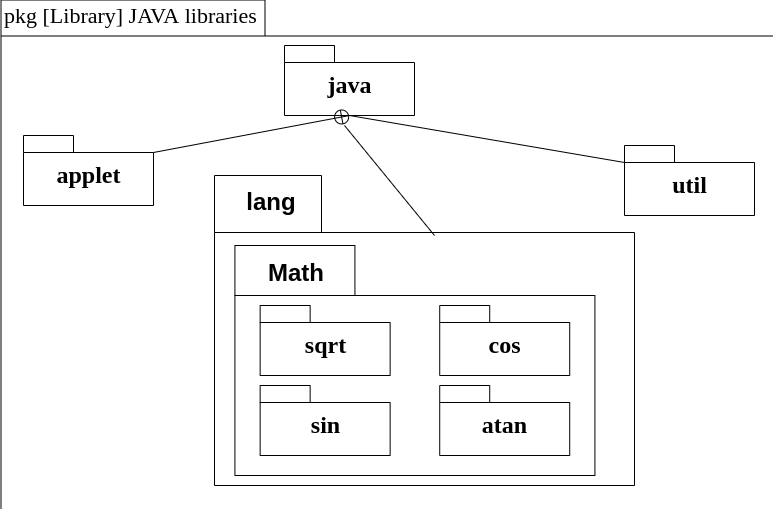
\includegraphics[width=0.75\textwidth]{figures/diagrama-pacote.png}
\caption{Diagrama de Pacote de parte da linguagem Java}
\label{fig:package_diagram}
\end{figure}